\section{The Test Setup}
The test setup is an arena with the dimensions 113 x 141 cm as can be seen in figure \ref{fig:testsetup}. The arena is divided into grid cells of 1x1 cm. An obsticle is placed in  the arena to create a a asymmetric map. This enables the robot to locate itself and drive towards a set goal. The map can be seen in figure \ref{fig:map} along with a cost map in figure \ref{fig:costmap} that is used for planning.
\begin{figure}[H]
\centering
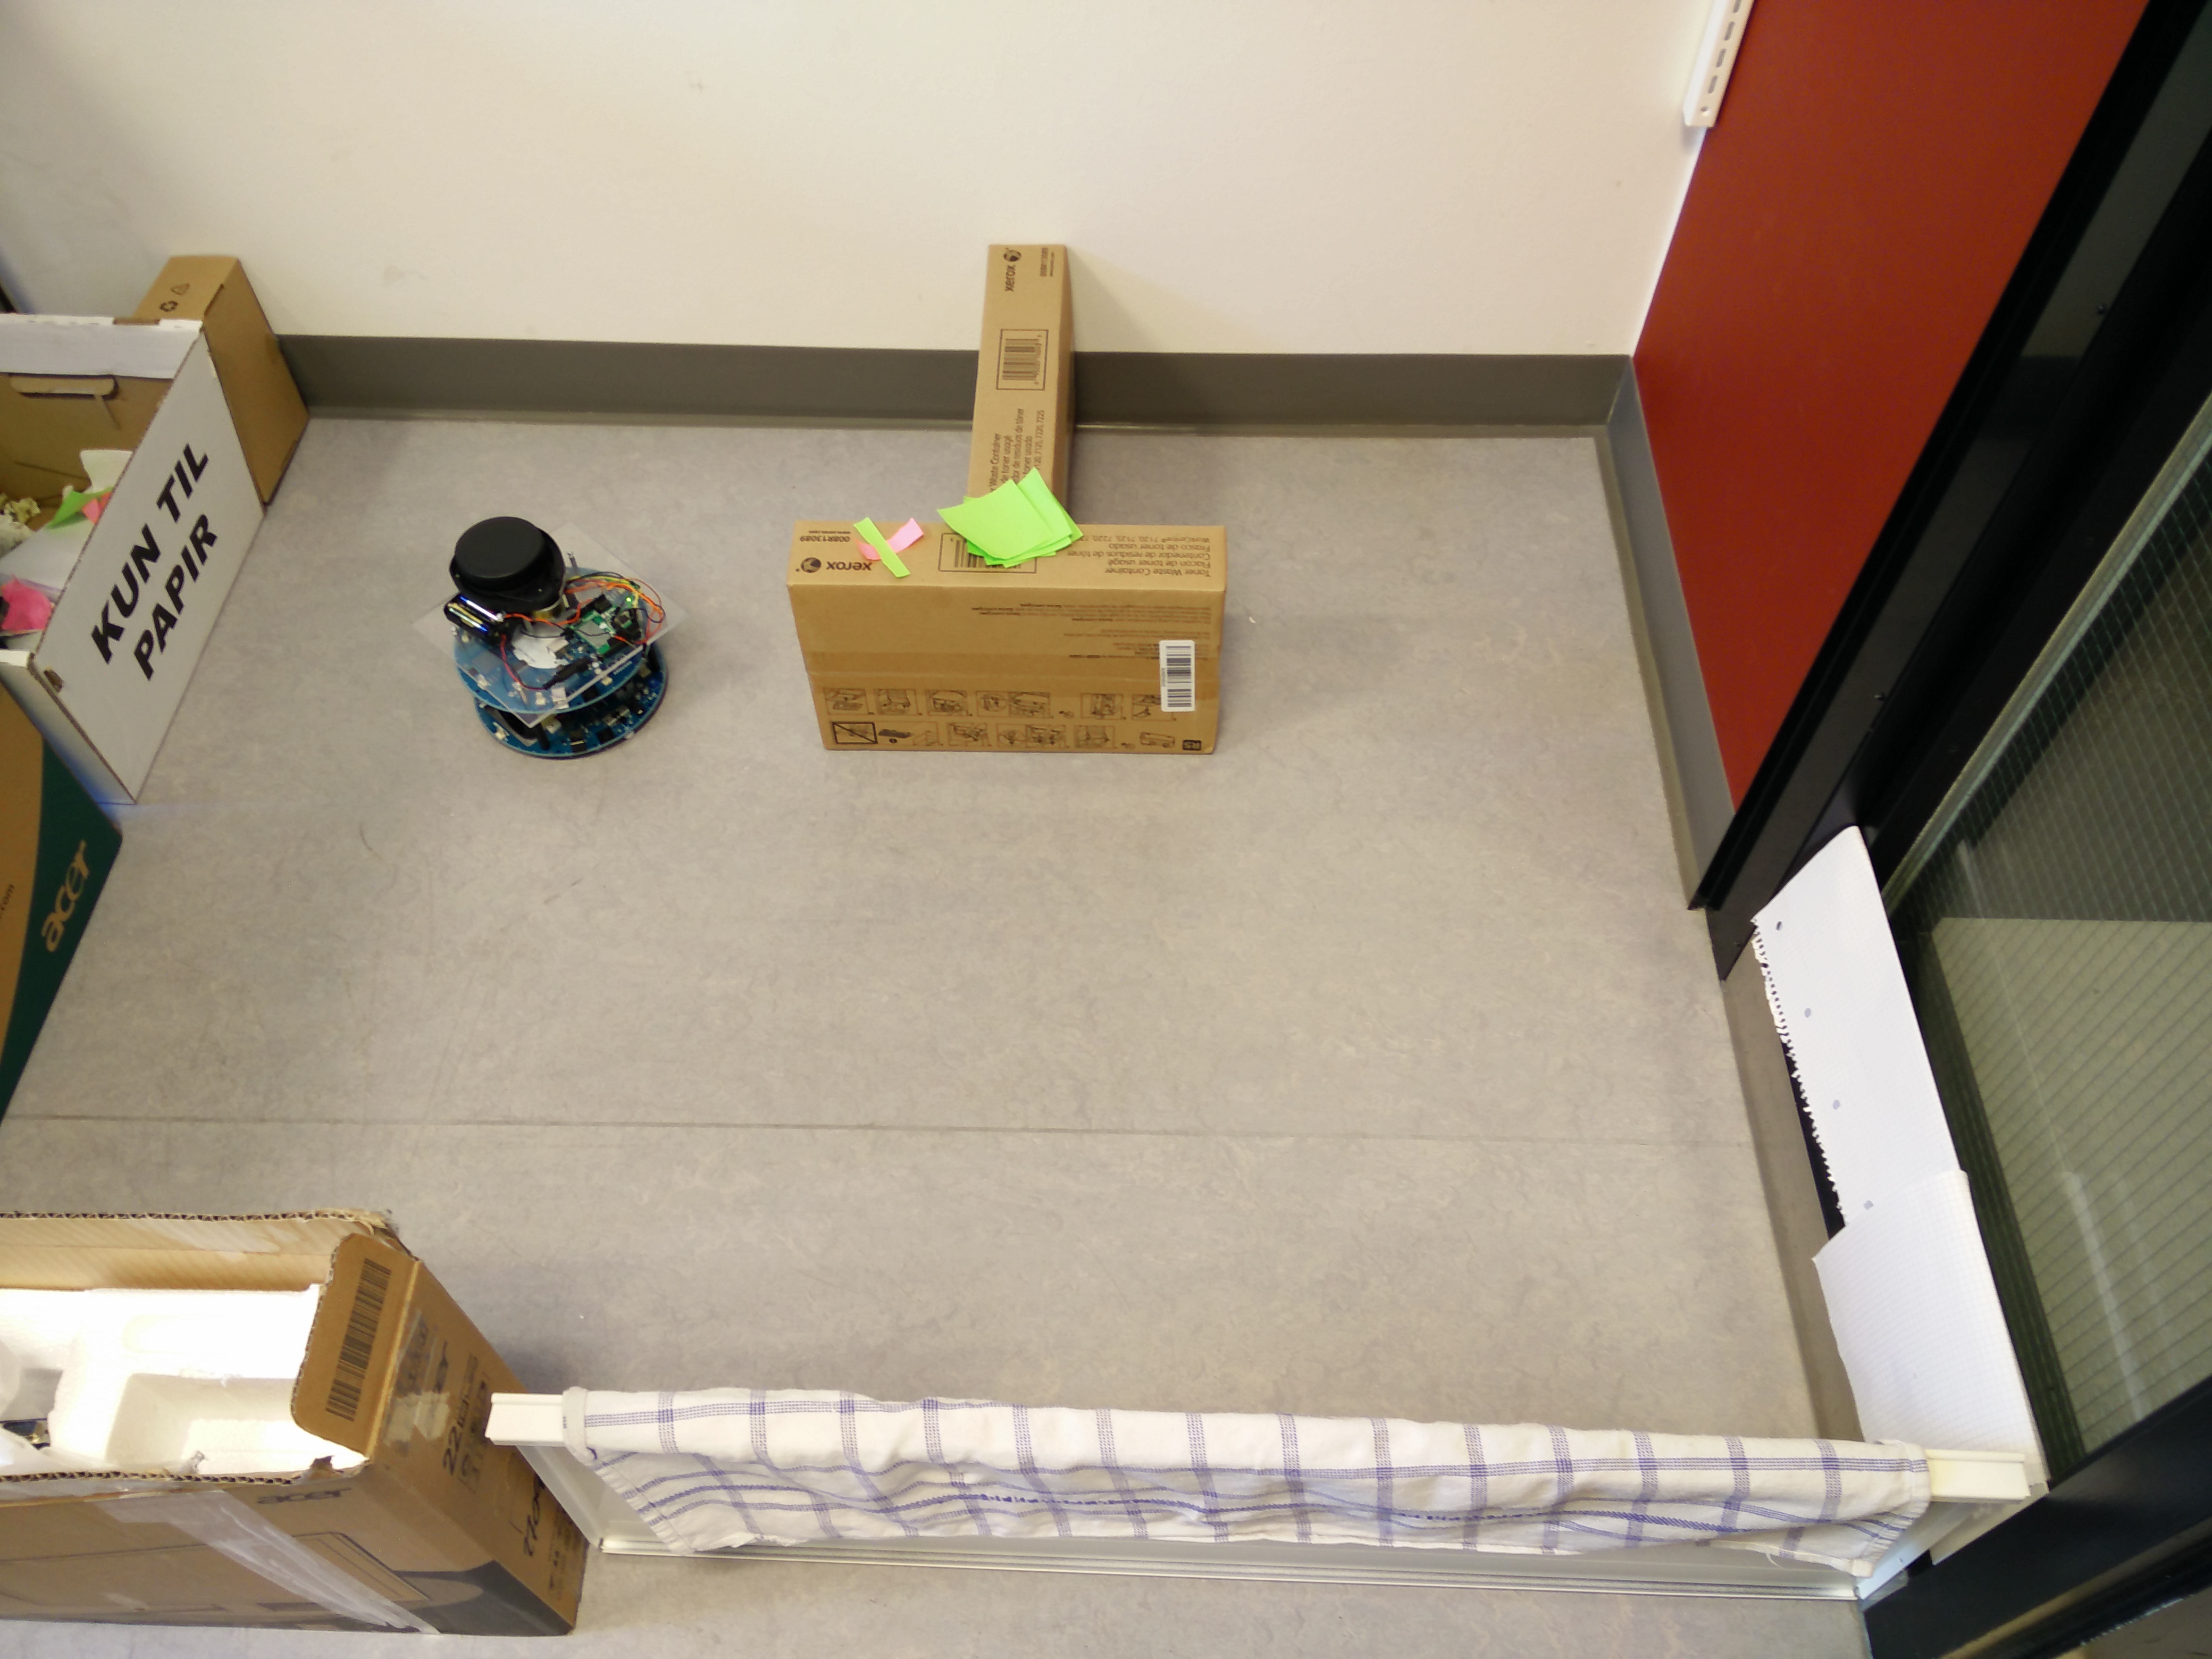
\includegraphics[width=0.8\textwidth]{billeder/testsetup}
\caption{Test Setup}
\label{fig:testsetup}
\end{figure}

\begin{figure}[H]
    \centering
    \begin{minipage}{.5\textwidth}
        \centering
        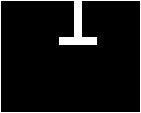
\includegraphics[width=0.6\textwidth]{billeder/map}
		\caption{Test map}
		\label{fig:map}
    \end{minipage}%
    \begin{minipage}{0.5\textwidth}
        \centering
        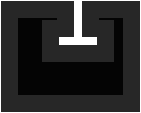
\includegraphics[width=0.6\textwidth]{billeder/costmap}
		\caption{Test cost map}
		\label{fig:costmap}
    \end{minipage}
\end{figure}
